\section{Implementation}

\subsection{Data Model Language}

A UML metamodel for the data model language is shown in
Figure~\ref{fig:datamodellanguage}. 


The key concept behind the language is that of a datamodel, a
datamodel is a model composed of dataclasses and dataelements which
holds structured data in a particular subject area. The \emph{models
  catalogue} toolkit is essentially a registry for these
\emph{datamodels}, each one being registered with a version
number. The datamodel maintains the structure and relationships
between a set of dataclasses and dataelements, each of which
essentially represent a \emph{data concept}. Dataclasses are in
essence very similar to \emph{entities} in entity-relational diagrams,
and to \emph{classes} in object-orientated programming; they are
simply data-structures. They can be composed from other dataclasses,
or from dataelements. Dataelements are atomic entities which can
represent a concept or a component of a concept, they can exist in a
datamodel independently or as a compositional attribute inside a
dataclass. 

We have a built a version of the language using the Eclipse Modelling
Framework (EMF ~\cite{EMF}), basing the various entities on
Ecore~\cite{ECORE} classes. A simplified overview model, without
attributes and methods, showing the Ecore model for this DSL is shown
in Figure \ref{fig:mcSimplifiedOverview}.

%%------------REDO-----------------------%%

\begin{figure}[here]
  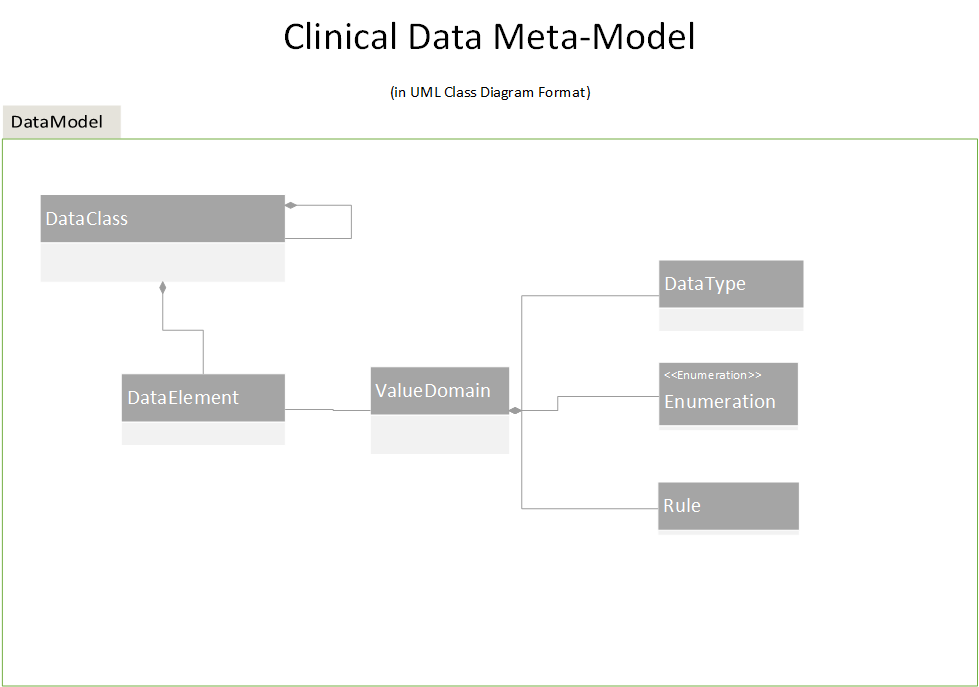
\includegraphics[width=0.5\textwidth,natwidth=610,natheight=642]{MetaModel}
  \caption{Overview of Metamodel} 
  \label{fig:mcSimplifiedOverview}
\end{figure}

\subsubsection{DataModel}

A datamodel is a grouping or containment entity which groups a set of
\emph{DataClasses} together. DataModels can be thought of as datasets,
or even database schemas, very often in the medical domain they are
defined either by XML Schema definition files, or by equivalent
schemas written in Excel.  DataModels are collections of
\emph{ConceptElements} which in turn can be either \emph{Data
  Elements} or \emph{Classes}. There is no real notion of composition
or multiplicity, a instance of a DataModel can contain an instance of
a Data Element or not as required by the instance.  DataModels are
named, have a description and have a version identity.

\subsubsection{DataClass}

A DataClass is a grouping or collection of \emph{attributes} which can
be data elements or classes, the attributes are currently
\emph{mandatory}, so that DataClass with 5 attributes must have those
5 attributes instantiated in an instance for it to be considered of
that DataClass. A DataClass in our meta-modelling language is so named
to differentiate it from the term \emph{Class} as used in object
oriented programming languages, the main difference being that it
captures the structural rather than behavioural aspects of a class.
DataClasses represent \emph{Concepts}, and can be \emph{Generalized}
into a hierarchy, giving some of the benefits of inheritance to the
language. In essence it enables users to take dataclasses from one
datamodel, build a sub-class with all the previous data points and
then add to it with new dataclasses and dataelement.
\subsubsection{Data Elements} 
Data Elements can also represent \emph{Concepts} and are by their nature \emph{atomic}.  Each data element is related to a value domain on a one-to-one basis, and the relationship is a two-way relationship.
\subsubsection{Value Domain}
A Value Domain is the domain in which the data element is represented, it can consist of one or more \emph{ValueSpecs}. In addition a valuedomain can have zero or more \emph{Measurement Units}, which are descriptive tags which refer to a measurement unit such as kilometers per hour, imperial pounds, or meters. 
\subsubsection{ValueSpec}
ValueSpecs are intermediate entities to describe \emph{how} the data will be represented. There are 3 ValueSpecs, the first is a \emph{datatype}, the second is an \emph{enumeration} of a datatype, and the last is a \emph{rule}. A valuedomain will have at least one ValueSpec and at most 3 ValueSpecs which must be of different kinds.
The main reason for creating a language for handling the data structures in this manner is not only so that models can be curated, versioned and maintained easily, but that the datamodels produced can then be transformed automatically for use in other heterogeneous systems. To illustrate this figure ~\ref{fig:mofLayers} shows the LEMMA meta-model within a 4 tier abstraction diagram. The layers within this diagram are based around idea put forward by the  OMG(~\cite{OMG}), specifically model driven architecture (MDA ~\cite{MDA}). The MDA defines \emph{n} abstraction layers for modelling, although 4-layers are normally used.
\begin{figure}[here] 
	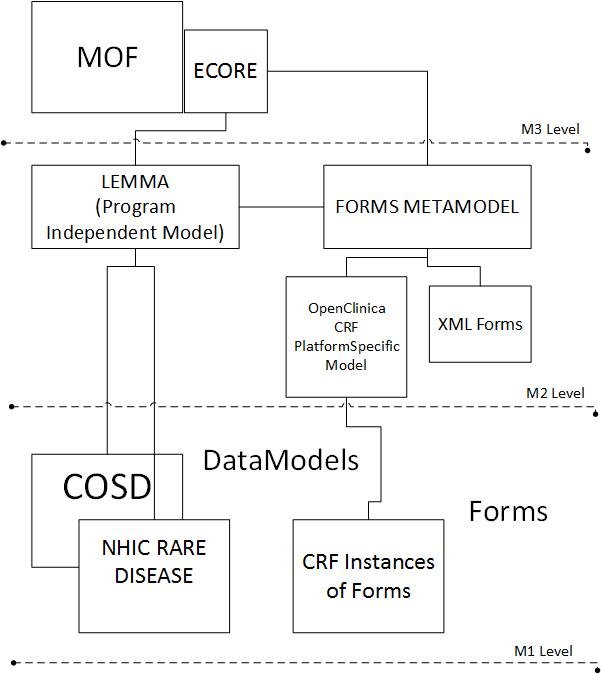
\includegraphics[width=0.5\textwidth,natwidth=610,natheight=642]{MOFLayers}
	\caption{ Datamodel in Excel Format} 
	\label{fig:mofLayers}
\end{figure}
The M0 layer is \emph{real-world} level, the level at which real world objects exist, people, cars, programs, etc. The M1 layer is level at which programs, such as a java program, or a java class definition exist in their static runtime form. The instantiation of a class occurs at the level below the class, so a java object runs in level M0. In defining datasets or datamodels we are dealing in datamodels which are instantiated at the M1 level, the \emph{Cancer and Outcomes Services Dataset} exists at this level, although their may be many conforming instances running at the M0 level. The datamodel is defined in out meta-modelling language, which exists at the M2 or meta-modelling level, and in turn conforms to the more abstract specification known as ECore.

An instance of a datamodel can be written in this DSL in the same way as java code, and figure \ref{fig:excelCOSD} shows how this code looks in the eclipse development toolkit. In this diagram the excel representation of the \emph{Cancer and Outcomes Services Dataset} shown in figure \ref{fig:excelCOSD} has been transformed into the meta-model.

\begin{figure}[here]
	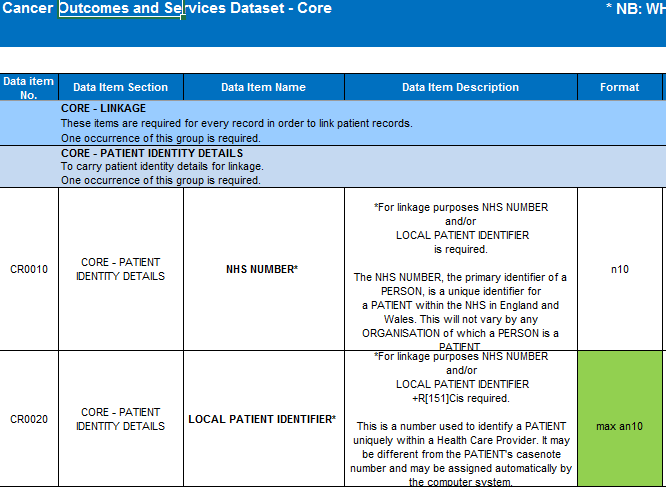
\includegraphics[width=0.5\textwidth,natwidth=610,natheight=642]{COSDExcelS}
	\caption{ Datamodel in Excel Format} 
	\label{fig:excelCOSD}
\end{figure}
The DSL is used to represent a model for Cancer data (part of the Cancer Outcomes and Services Dataset ~\cite{COSD}) in figure \ref{fig:elmcosd}, and is being used within the eclipse toolkit. The DSL can be used to transfer datasets between instances of the models catalogue, although other formats such as JSON and XML are also available.

\begin{figure}[here]
	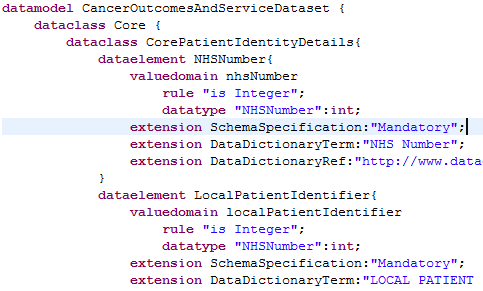
\includegraphics[width=0.5\textwidth,natwidth=610,natheight=642]{MCCOSDModelS}
	\caption{ Datamodel in Eclipse environment} 
	\label{fig:elmcosd}
\end{figure}

\subsection{Metadata Registration}

In designing the language, we gave due consideration to the ISO/IEC
11179 standard for metadata registration.  This standard sets out a
metamodel for data definitions, together with a set of processes for
their registration and publication.   

Refer also to the CancerGrid project \cite{crichton2009metadata}. 

\begin{figure}[here]
  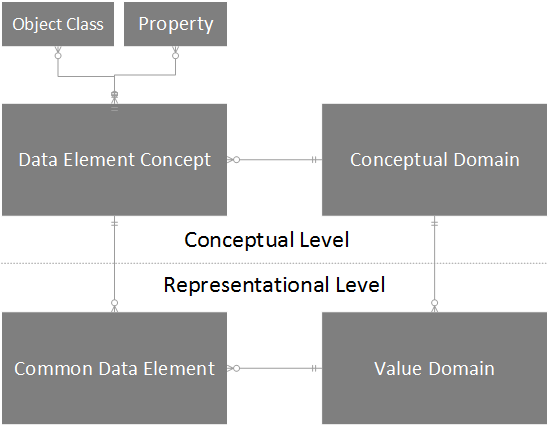
\includegraphics[width=0.48\textwidth,natwidth=610,natheight=642]{BasicISO}
  \caption{Core model for ISO11179 Metadata Registry} 
  \label{fig:basicMDR}
\end{figure}

The ISO11179 standard uses the notion of a \emph{data element
  concept}, \emph{a data element}, \emph{a value domain}, and a
\emph{conceptual domain}. The standard currently confines itself to
the detailed level of concepts and data elements and has no notion of
collections of data elements or data element concepts, but instead
attaches two attributes: an \emph{object class} and a \emph{property}
to each data element concept and these attributes allow the data
element concept's to be aggregated or classified. This core model of
the ISO11179 is illustrated in figure \ref{fig:basicMDR}. The data
element concept and conceptual domain entities belong to the
\emph{conceptual level} whilst the common data element and value
domain both belong to the \emph{representational level}.

For example an Integer data-type in a programming language may be used
to represent inches in a measurement program, it may also be used to
count vehicles in a logistics application.  A data element is said to
be comprised of a data element concept(DEC) which is its meaning and a
value domain(VD) which is its representation.

\begin{table}[h]
  \begin{tabular}{ p{1.8cm} p{2.8cm}  p{3.0cm}  }  % centered columns (2 columns)
    \hline
    Entity & ISO Definition & ISO11179 Implementation Guidelines  \\ 
    \hline
    Data Element Concept(DEC) & An idea that can be represented in the form of a data element, described independently of any particular representation. & A concept that can be represented in the form of a Data Element, described independently of any particular representation.\\
    Common Data Element(CDE) & A unit of data for which the definition, identification, representation, and permissible values are specified by means of a set of attributes. & A unit of data for which the definition, identification, representation and Permissible Values are specified by means of a set of attributes. \\
    Value Domain (VD) & The description of a value meaning. & A description of a Value Meaning. \\
    Conceptual Domain (CD) & A set of valid value meanings, which may be enumerated or expressed via a description.& A set of valid Value Meanings.\\
		\hline
  \end{tabular}
\end{table}

The table lists the definitions of the key entities used in the
standard Conceptual domains comprise sets of value domains, they
provide a collection mechanism of \emph{Value Meanings} which provide
representation for a particular data element concepts. Data Element
Concepts can then be grouped according to their Object Class, or
Property, however whilst this works for a system that is focussed
entirely on the metadata units, any working software system will need
to group the data elements in a structure that is easily transformed
into the components such as Classes and Entities that are used in most
information systems.


\subsection{Forms and Automatic Software Generation}

By defining the LEMMA metamodel and a similar and dependent Forms
metamodel, both at the M" level, and both \emph{Platform Independent}
we are able to relate curated data elements to forms elements, and by
selecting a group of dataelements and dataclasses automatically
generate a set of related forms. This can be done in several ways, the
most used way is to generate a platform independent model and then use
that model to generate an Excel template.

The Models Catalogue, like many software developments, evolved from a
mix of requirements on a number of different projects.  Initially a
metadata registry was built using an XML database, however problems
were encountered with scalability.  Most of the language and metamodel
developments were carried out using XText and the Eclipse Modelling
Framework, resulting in a usable java code base, however usability
requirements neccessitated the refactoring of this software using a
stack consisting of Grails and Angular JS.

Grails is built on the Spring framework, which is not only proven to
be very robust and scalable, but is also relatively easy to implement
and so enables quick agile development cycles. Previous
implementations using Java/Spring and Java/Roo have proved very
time-consuming to experiment with, whereas Grails has proven to be
more flexible and easier to experiment with.  Domain specific
languages (DSL’s) can be built on this framework, and this capability
offered scope to build a DSL based on the LEM DSL specification and
meta-model expanded in the previous section.
 
The front end user interface was implemented using a combination of
HTML with Javascript and CSS, the principal framework used being
Angular JS. Communication with the client was carried out using a REST
controller, enabling a variety of clients potentially to link up with
the Model Catalogue.

GORM was used as a persistence mechanism, with a MySQL relational
database as storage, although different GORM adapters made it possible
to attach NO SQL datastores such as Neo4J and MongoDB. The full
architectural stack is shown in
Figure~\ref{fig:ApplicationArchitectMDR}

\begin{figure}[here]
  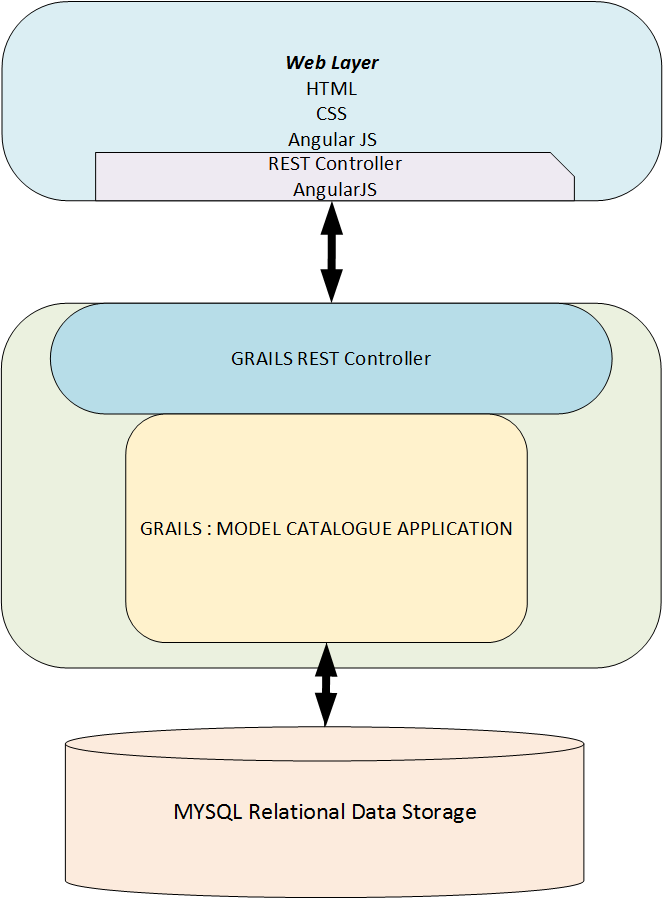
\includegraphics[width=0.48\textwidth,natwidth=610,natheight=642]{ApplicationArchitect1}
  \caption{Overview Architecture} 
  \label{fig:ApplicationArchitectMDR}
\end{figure}

The Grails/GORM framework enabled the Ecore model to generate the
basic Grails Domain model, and from that a Groovy DSL was built, using
the Builder pattern, to handle transformations internally between
different representational languages such as XML and Excel. A series
of importers was built for data input from Excel, CSV, and various XML
variants. Most XML structures are handled by transforming the XML from
its native structure to our internal DSL-based XML structure.

The internal domain model used a basic \emph{Catalogue Element} which
was able to link elements via the \emph{relationship} and
\emph{relationshipType} classes. The core language model discussed
earlier has been enhanced to by allowing user-defined relationships to
be added to the core model. Any catalogue element is able to be
related to any other catalogue element through a relationship class,
this relationship is constrained by the relationshipType object which
can prevent different catalogue element types being related, so that a
Model cannot directly be related to a say a Datatype
Enumeration. Relationship types can be added to the Model dynamically,
so that even though the relationship between a Model and Datatype
enumeration is prevented initially, a new type could be introduced by
an administrator or super user to add in that relationship. The
EMF-based tools to automatically generate the whole Models Catalogue
code-base using Groovy/Grails/Angular were not available at the start
of the project, and although work has been undertaken to build such a
toolkit it not yet complete.

The following subsections describe the basic use cases for the Model
Catalogue, and how these use cases were implemented.

\subsection{Listing of DataModels}

The key use case required in both projects was the ability to catalogue a set of data elements and data classes so that different schema could be compared and curated. Listing is currently carried out using a REST interface which is queried using an Angular client. Figure \ref{fig:treeviewOfDataModel}
\begin{figure}[here]
	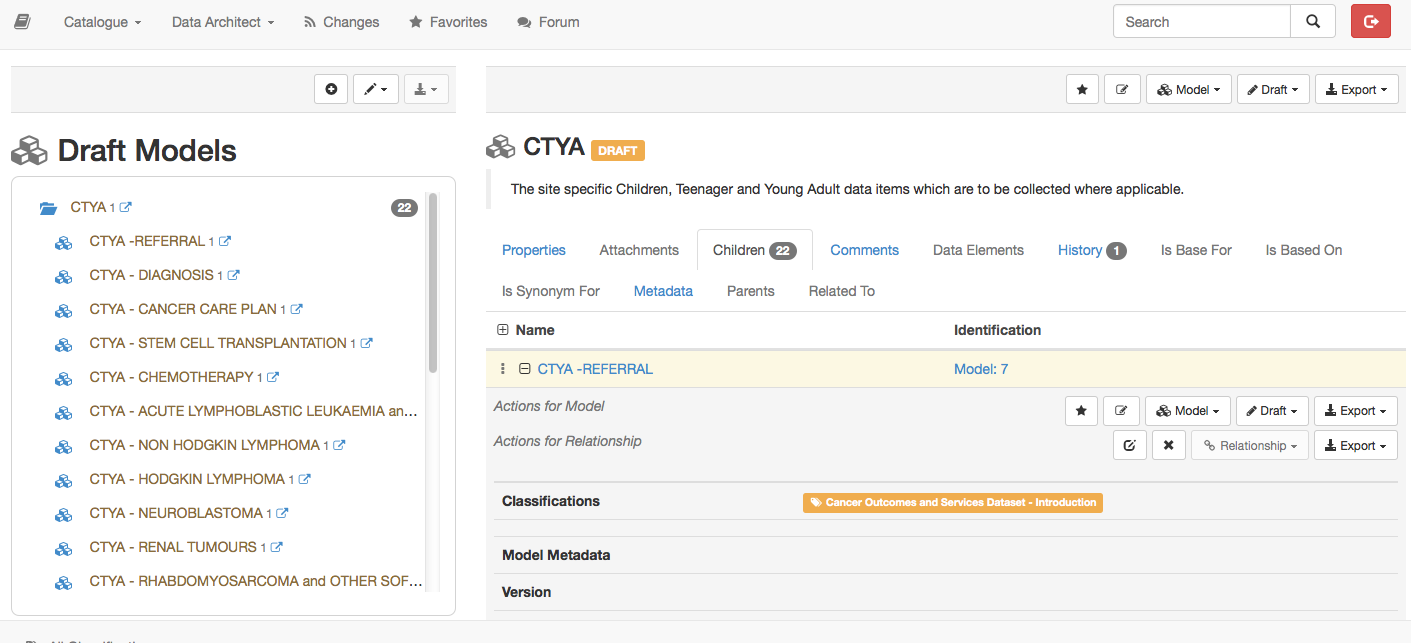
\includegraphics[width=0.5\textwidth,natwidth=610,natheight=642]{DataModelTreeView}
	\caption{Screen Shot of DataModel Listing} 
	\label{fig:treeviewOfDataModel}	
\end{figure}

\subsection{forms}

Typically the initial data models are entity-centric: for example
cancer models are initally built around the entities of
\emph{Patient}, \emph{Tumour}, etc.  Forms are typically structured around
events: \emph{Registration}, \emph{Surgery}, etc.  We construct
separate models for forms, re-using the elements from the
entity-centric model, thus providing a different view upon the same
data.  (As as aside, the Patient Pathway models interact with these
forms models, providing a workflow, ordering form completion).

With respect to forms, we take an approach analagous to that of the
Model-Driven Architecture~\cite{MDA-proposal}: that of
Platform-Specific Models (PSMs) and Platform-Independent models
(PIMs).  Our platform-independent model in this regard is based on the
emerging ISO standard for forms~\cite{ISOForms}.  This provides
structure in terms of \emph{sections}, \emph{sub-sections},
\emph{repeating groups}, and so on, but is not specific to any
particular implementation.  The model is based on previous work on
domain-specific languages for forms~\cite{Abler2011}.

Our initial platform-specific target is \emph{OpenClinica}, a tool for
supporting data capture for clinical trials.  OpenClinica forms are
created using a model supplied in Excel Spreadsheet format.

Our generation of XML schema may also be seen as a platform-specific
implementation of the forms model.  XML schema are used to define
message structures, and have a similar structure to the OpenClinica
forms, although typically additional data is required in XML schema -
context such as the patient for which the data is about, or the person
submitting the data; or linking information which may be automatically
created during manual input into a web interface. 


\subsection{selection of data elements for form generation}
For many clinical users one of the key requirement was the ability to generate forms for clinical research which were generated form a single authorative source, and the ability to take data elements, manage them to build a form and then output either a form or an XML representation for use in another system, such as OpenClinica was key to the work carried out. 



\subsection{relationships between 2 DataModels}
Very often different research groups will arrive at slightly different models for the same or very similar diseased, so another use case for the Models Catalogue was the ability to compare different Data Models, Data Classes and individual Data Elements.






%%-------------------------------
%%Drop next section
%%------------------------------
%%Some of the main relationships that are currently modelled in the \emph{Models Catalogue} are as follows:
 %%
%%\begin{center}
%%	\begin{tabular}{ p{1.5cm}  p{1.5cm}  p{1.5cm}   }  % centered columns (5 columns)
%%		Source & Relationship & Destination  \\
%%		Model & containment & DataElement   \\
%%	    Model & containment & Class    \\
%%	    Model & hierarchical & Model  \\
%%	    DataElement & supersession & DataElement  \\          
%%	\end{tabular}
%%\end{center}
%%
%%The Core architecture can seen in figure\ref{fig:ApplicationArchitectMDR} 
%%
%%\begin{figure}[here]
%%	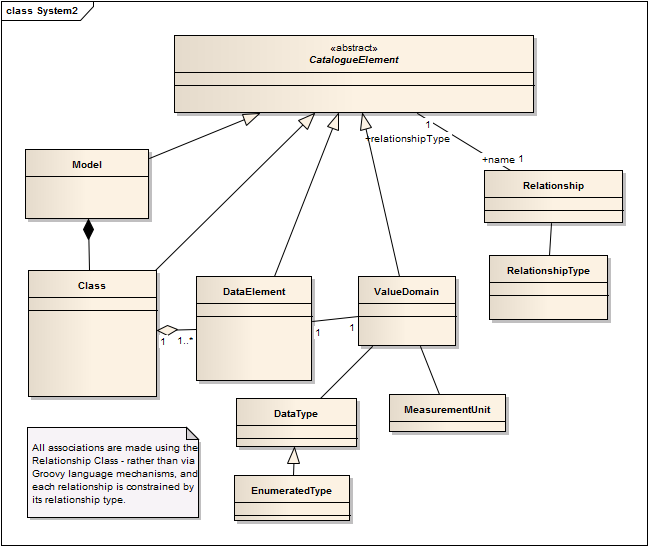
\includegraphics[width=0.5\textwidth,natwidth=610,natheight=642]{System2}
%%	\caption{Overview Architecture} 
%%	\label{fig:System2MDR}
%%\end{figure}
%% 
\subsection{Modelling Overview}





 
 